
%1
\section{はじめに}

% \footnotetext{}



%1.2
\subsection{問題設定}
辺の長さが与えられた無向グラフ $G = (V,E)$ の上を
1人または複数人の巡査が一定の速さで動きながら各点を警備する.
各点 $v_i \in V$ には周期 $q_i$ と利得 $p_i$ が与えられている.
ある点を警備できているとは,どの連続した2回の訪問も間隔がその点の周期以内であることを言う.
グラフ $G$ と巡査の人数 $m$ が与えられたときに,
$m$ 人の巡査により警備される点から得られる利得の合計を最大化するのが目的である.
これに関連して,全ての点を警備できる最小の巡査の数を求める巡査数最小化問題も考える.
前者を \maxprofit, 後者を \minpatroller と呼ぶことにする.
\minpatroller では利得は無関係となる.

巡査は2人以上同時に1つの点に存在してもよいし,
1つの点は複数人の巡査により交代で訪問して警備してもよいとする.

巡査は点を訪問するときに一定時間そこにとどまる必要があるという問題も考えられるが,
後で説明するようにグラフを変形することによりこの拘束時間は $0$ である問題に帰着できる.



%1.3
\subsection{記号の定義}
\begin{itemize}
	\item $G = (V,E)$ : 無向グラフ.
	\begin{itemize}
		\item $V = \set{ v_1, v_2, \ldots, v_n }$
		\begin{itemize}
			\item $p_i$ : $v_i$ を警備することにより得られる利得.
			$p_i \leq 0$ の点は最初に除外してよいので $p_i > 0$ であるとする.
			\item $q_i$ : 周期.
			% この時間以内に巡査が $v_i$ に帰ってこないと $v_i$ を訪問したことにならない.
			どの連続した2回の点 $v_i$ の訪問も間隔が周期 $q_i$ 以内であるとき
			この点 $v_i$ を警備していると定義する.
			$q_i \geq 0$.
			% \item $w_i$ : $v_i$ を訪問したときにそこにとどまる必要がある時間(拘束時間).
			% $w_i \geq 0$.
		\end{itemize}
		\item $E \subseteq V \times V$. 辺 $(v_i, v_j) \in E$ を $e_{ij}$ とも書く.
		\item $d(e)$ : 辺 $e \in E$ の重み(長さ).
		$e = (v_i, v_j)$ に対し $d(v_i,v_j)$ や $d_{i,j}$ のようにも表す.
	\end{itemize}

	\item 巡査 : $S = \set{ s_1, \ldots, s_m }$
	\begin{itemize}
		\item 速度 $1$ 以下で辺上を動く.
		\item $V_{s_i} \subseteq V$ : 巡査 $s_i$ が警備する点の集合.
		\item $V_S     \subseteq V$ : $\dbigcup_{s_i \in S} V_{s_i}$. 
		巡査 $s_i \in S$ が警備する点の集合の和集合.
	\end{itemize}
\end{itemize}



%1.4
\subsection{形状}
本稿では以下の形状について考察する.

\begin{itemize}
	\item Line    : $E = \setmid{ (v_i, v_{i + 1}) }{ 1 \leq i \leq n - 1 }$ ,
	一直線上に点が並んだグラフ.
	\item Star    : $E = \setmid{ (v_i, 0) }{ 1 \leq i \leq n }$ ,
	全ての枝の端点の一方が根であるような木.
	\item StarC   : Star で辺の長さが全て等しい場合.
\end{itemize}




%2


\section{結果一覧}
以下に現在確かめられている計算複雑性を示す.
巡査数 $1$ と $\geq 1$ はそれぞれ \maxprofit で $m = 1$, $m \geq 1$ の場合を表し,
MIN は \minpatroller を表す.

\minpatroller において,
点と同数の $n$ 人巡査がいれば明らかに全点を警備できることから,
\maxprofit を $m = 1$ から $n$ までの場合について順に解き,
初めて全点を警備できたとき(最大化した利得が $\dsum_{i = 1}^n p_i$ に等しいとき)
の $m$ により求められるので,\minpatroller は
複数の巡査の場合の \maxprofit に多項式時間帰着可能である.

周期 $Q$ は,全ての点の周期が等しい場合, $\geq 0$ はそうでない場合を表す.
利得 $1$ は,全ての点の利得が等しい場合
(単に点の数を最大化する問題に相当するため $p_i = 1$ としてよい),
$> 0$ はそうでない場合を表す.


太字の部分を証明することにより他の部分を決めることができる.
Pは多項式時間算法あり,NPHはNP困難,?の部分は未解決であることを表す.

\begin{table}[htbp]
	\centering
	\caption{警邏問題の計算複雑性一覧\label{tab:Patrol}}
	\begin{tabular}{|c|c|c||c|c|c|c|c|}
	\hline 周期 & 利得 & 巡査数 & Line & StarC & Star & General \\
	\hline $Q$      & $1$   & $1$      & P             & P             & {\bf P }  & {\bf NPH} \\
	\hline $Q$      & -     & MIN      & P             & P             & {\bf NPH} & NPH \\
	\hline $Q$      & $1$   & $\geq 1$ & P             & P             & NPH       & NPH \\
	\hline $Q$      & $> 0$ & $1$      & P             & P             & {\bf NPH} & NPH \\
	\hline $Q$      & $> 0$ & $\geq 1$ & {\bf P}       & {\bf P}       & NPH       & NPH \\
	\hline $\geq 0$ & $1$   & $1$      & P             & ? ($\star 2$) & {\bf NPH} & NPH \\
	\hline $\geq 0$ & -     & MIN      & ? ($\star 1$) & ? ($\star 2$) & NPH       & NPH \\
	\hline $\geq 0$ & $1$   & $\geq 1$ & ?             & ? ($\star 2$) & NPH       & NPH \\
	\hline $\geq 0$ & $> 0$ & $1$      & {\bf P}       & ? ($\star 2$) & NPH       & NPH \\
	\hline $\geq 0$ & $> 0$ & $\geq 1$ & ?             & ? ($\star 2$) & NPH       & NPH \\
	\hline
	\end{tabular}
\end{table}

また,?の部分についての考察中に得られた結果として,
最初の訪問時刻 $r_i$ が指定されていて,かつ訪問間隔が周期 $q_i$ ちょうど
でなければならないという問題設定にした場合,
$\star 1$ では擬多項式時間算法が存在し,
$\star 2$ ではNP困難となる.



\section{Line}

$G$ が Line の場合は実直線上に全ての点を置くことができるので,
% $x$ 軸上に点を置き, 
それぞれの座標を $x_1, x_2, \ldots, x_n$ とする.
また,添え字は $x_1 \leq x_2 \leq \cdots \leq x_n$ としておく.

\subsection{巡査が1人の場合}


\begin{theo}
	巡査1人, $G$ が Line の \maxprofit には多項式時間算法が存在する.
	\label{theo:PatrolonLine_1}
\end{theo}

\begin{lemm}
	ある実行可能解 $A$ があったとき,
	$A$ で巡査が警備している最も左の($x$ 座標の小さい)点 $v_l$ と
	最も右の点 $v_r$ について,
	区間 $[x_l, x_r]$ を往復する動きにより $A$ と同等以上の利得を得ることができる.
\end{lemm}

\begin{proof}
	$A$ で巡査 $s$ が警備している点の集合を $V_s$ と書く.
	$x_i < x_j$ であるような任意の $v_i, v_j \in V_s$ について,
	$v_i$ を訪問した後 $v_j$ を訪問し再び $v_i$ に戻るまでの時間について,
	$v_j$ と $v_i$ の間の移動時間の最小値は片道 $x_j - x_i$ なので,
	点 $v_i$ を $q_i$ 以内に訪問できていることから,
	行き帰りの時間について,
	\begin{equation}
		2(x_j - x_i) \leq q_i
	\end{equation}
	が成り立つ.
	% 点 $v_j$ についても同様に
	% \begin{equation}
	% 	2(x_j - x_i) \leq q_j
	% \end{equation}
	% となる.
	$x_i < x_j$ であるような $v_i, v_j \in V_s $ は任意に選んでいたので
	% \begin{equation}
	% 	\sforall v_i, v_j \in V_s . \lr{
	% 		2(x_j - x_i) \leq q_i \AND 2(x_j - x_i) \leq q_j
	% 	}
	% \end{equation}
	$x_i$ を基準に考えると
	\begin{equation}
		\sforall v_i \in V_s . \lr{
			\sforall v_j \in V_s . 
			\lr{ 2(x_j - x_i) \leq q_i }
		}
	\end{equation}
	すなわち
	\begin{equation}
		\sforall v_i \in V_s . \lr{
			\max_{v_j \in V_s} 2(x_j - x_i) \leq q_i
		}
	\end{equation}
	$v_l$, $v_r$ のいずれかが $x_i$ から最も遠い点となるので
	\begin{equation}
		\sforall v_i \in V_s . \lr{
			\max( 2(x_i - x_l), 2(x_r - x_i) ) \leq q_i
		}
		\label{eq:PatrolonLine_2}
	\end{equation}
	ここで,$v_r$ と $v_l$ を往復する動きを考えると,これは式\Ref{eq:PatrolonLine_2}を満たすので
	$V_s$ に含まれる点全てを警備することができる.
\end{proof}

以上により, 巡査1人の Line では2点間を往復する動きのみ考えれば良いことが分かったので,
$\dbinom{n}{2}$ 通りの両端を選び,その区間に含まれる点 $x_i$ について
$\max( 2(x_i - x_l), 2(x_r - x_i) ) \leq q_i$ を満たすものを警備するときの利得の合計を
比較することで $O(n^3)$ で最適解を得ることができる.
\qed \Ref{theo:PatrolonLine_1}.

これについてはCoeneらが
$O(n^2)$ で最適解を得る算法を与えている~\cite{coene2011charlemagne}.




\subsection{巡査が複数の場合}

巡査が複数人の場合,それぞれの能力は同じなので,
巡査がすれ違うような動きはお互いの動きを交換し引き返すような動き方にすることができる.
これにより,巡査は初期配置の $x$ 軸上の順番を保って動くとしてよいことが言える.
ある実行可能解 $A$ についてこのような変換を行ったものを $A^*$ と表すことにする.


\subsubsection{周期が全て等しい場合}
まず周期が全て等しい場合を考える.
この場合,同じ位置に複数の点が存在するとき,どれか1つを警備できるならば全て警備できるので,
それらの合計の利得をもつ新たな1つの点にまとめることができる.
よってここでは $x_1 < x_2 < \cdots < x_n$ となっているとして進める.


\begin{theo}
	\label{theo:MultiplePatrolOnLine_1}
	巡査が複数人, $G$ が Line, $q_i = Q$ の \maxprofit には多項式時間算法が存在する.
\end{theo}

初めに次の補題を示す.

\begin{lemm}
	\label{lemm:MultiplePatrolOnLine_3}
	ある巡査 $s$ 1人のみにより警備されている点 $x_i$ が存在するとき,
	$s$ が動ける範囲は $\abs{ x - x_i } \leq q_i / 2$ となる.
\end{lemm}

\begin{proof}[Proof of \Ref{lemm:MultiplePatrolOnLine_3}]
	もし $s$ が $\abs{ x_{out} - x_i } > q_i /2$ であるような位置 $x_{out}$ に
	行くことがあるとすると,
	$s$ が最後に $x_i$ を出発してからの時間と,
	次に $x_i$ に戻るまでの時間を合わせた時間 $t$ は
	\begin{equation}
		t > 2 \abs{ x_{out} - x_i} > q_i
	\end{equation}
	となり,
	$x_i$ は $s$ 以外の巡査により訪問されていないので
	$x_i$ を警備できていないことになり矛盾する.
\end{proof}



\begin{lemm}
	\label{lemm:MultiplePatrolOnLine_2}
	巡査が複数, $G$ が Line, $q_i = Q$ の警邏問題に対するある実行可能解 $A$ について,
	各巡査がそれぞれ独立で両端に点があるような区間を往復する実行可能解であって
	$A$ 以上の利得を得られるようなものが存在する.
\end{lemm}

\begin{proof}[Proof of \Ref{lemm:MultiplePatrolOnLine_2}]
	$A$ で警備する点の集合を
	$V_S = \set{ v_1', v_2', \ldots, v_k' }
	 \quad (  x_1' < x_2' < \cdots < x_k'  )$
	とする.
	$A$ は巡査の初期順序を保つ動き $A^*$ に変換してあるとし,
	それらを $x$ 軸上の左側から $s_1, s_2, \ldots, s_m$ とする.
	さらに,$x < x_1'$ を動くものはその時間 $x_1'$ で待機するようにしても損をしないため,
	全ての巡査は区間 $[x_1', x_k']$ を動くように変換できる($x_k' < x$ を動くものも同様).

	まず $x_1'$ に注目する.
	いま,巡査順序を保つ $A^*$ に変換しており,
	巡査は $x_1'$ より左には進まないように変換しているので,
	$x_1'$ に $s_1$ 以外の巡査 $s_i$ が訪れるときは必ず $s_1$ が $x_1'$ に存在することになる.
	よって,$s_1$ 以外の巡査は $x_1'$ を訪れずに $x_2' \leq x$ を動くようにしてよい.

	補題\Ref{lemm:MultiplePatrolOnLine_3}により $s_1$ の可動範囲は
	$[x_1', x_1' + Q/2]$ となるが,
	$s_1$ はこの区間を往復することによりこの区間に存在する全ての点を警備できる
	(巡査1人の Line での証明より)ので,
	この区間 $[x_1', x_1' + Q/2]$ を $s_1$ 以外の巡査が警備する必要はない.
	$V_S$ の点のうち
	$x_a$ を超えない最も左にある点の位置を
	$lm(x_a) := \dmin_{ \setmid{ x_i \in V_S }{ x_a \leq x_i } } x_i$, 
	$x_b$ を超えない最も右にある点の位置を
	$rm(x_a) := \dmin_{ \setmid{ x_i \in V_S }{ x_i \leq x_r } } x_i$, 
	と書くことにすると,
	$s_1$ は区間 $[x_1', rm(x_1' + Q/2)]$ を往復すればよく,
	$s_2, \ldots, s_m$ のうち
	$[x_1', x_1' + Q/2]$ の内部を動いていた巡査は
	他の巡査の動く範囲に交わらない適当な位置に待機させることで取り除き,
	$[x_1', x_1' + Q/2]$ に入ってくる巡査は
	$lm(x_1' + Q/2)$ でその時間待機するようにしてよい.

	このような変換の後,
	$lm(x_1' + Q/2)$ を警備している最も添え字の若い巡査を $s_j$ とすると,
	$s_j, s_{j + 1}, \ldots, s_m$ と区間 $[lm(x_1' + Q/2), x_k']$
	に存在する点について, $s_1$ のときと同様の変換をさらに行うことができる.
	これを最後まで繰り返すと,
	全ての巡査がそれぞれ両端に点が存在するような
	独立な区間を往復(または1点で停止)するような動きに変換できる.
	この変換で $A$ で警備していた点は全て警備できているので $A$ 以上の利得が得られている.
\end{proof}


以上により,各巡査の動きとしては
区間 $[x_i, rm(x_i + Q/2)]$ を往復するもののみを考えれば良いため,
$n$ 個の区間 $[x_i, rm(x_i + Q/2)] \quad (i = 1, 2, \ldots, n)$ から
$m$ 個の重複のない区間を選ぶことで最適解が得られる.
$n$ 個の区間 $I_i := [x_i, rm(x_i + Q/2)]$ について
その区間に含まれる点から得られる利得の合計 $P_i$ を求めておけば,
重み付き区間の選択問題で区間数 $\leq m$ の制限付きの場合を解くことになる.

まず $x_1, \ldots, x_n$ はソートしておく ($O(n \log n)$).
前半の $P_i$ の求め方だが,これは
$x_1, \ldots, x_n$ と $(x_1 + Q/2), \ldots, (x_n + Q/2)$ を
先頭から見て小さい方から1つずつ取り出していき,
\begin{itemize}
	\item $x_i$ なら $p \gets p + p_i$, 
	\item $x_i + Q/2$ なら $P_i \gets p$; $p \gets p - p_i$
\end{itemize}
という操作をしていくことで計算できる.
$p$ は今見ている長さ $Q/2$ の区間に含まれる点の利得の合計を表す一時変数で, 最初に $0$ で初期化する.



後半の,重複のない $m$ 個の区間を選び重みの和を最大化する問題は,
以下の漸化式\Ref{eq:MultiplePatrolOnLine_DP}に従う動的計画法で
$m \times n$ の表を左上から計算することにより $O(mn)$ で
最適な区間を選択できる.
$h(j)$ は,区間 $I_j$ より左にある交わらない区間のうち最も右にあるものの添え字を返すもので,
$1 \leq j \leq n$ について $O(n)$ の前計算で得られる.
$OPT(i,j)$ は,区間 $I_1, \ldots, I_j$ から 最大 $i$ 個の区間を選ぶときの
重みの合計の最大値を表す.
$OPT(m,n)$ が求めたい利得の最大値となる.
選ばれた区間も表をトレースバックすることにより再計算できる.

\begin{equation}
	\label{eq:MultiplePatrolOnLine_DP}
	OPT(i,j) = 
	\begin{cases}
		0 & \IF i = 0 \\
		\max
		\begin{cases}
			OPT(i,j - 1) \\
			P_j + OPT(h(j), i - 1)
		\end{cases}
		 & \IF i \neq 0 \\
	\end{cases}
\end{equation}

この算法の計算量は全体で $O(n \log n + nm)$ である.
\qed \Ref{theo:MultiplePatrolOnLine_1}.




\subsubsection{周期が異なる場合}

次に,周期が異なる場合を考える.
こちらは未解決であるが,この問題の難しさを示唆する例をいくつか示す.

点の周期が全て $Q$ であるときは,巡査は各々の区間を独立に往復すればよかったが,周期が任意の場合,
動く範囲に交わりがあり往復でもない動きが最適となる次ような例が存在する.
図\ref{tikz:multiserver_example}は
巡査の軌跡(各時刻 $t$ における巡査の位置 $x$ を表す関数 $f : t \mapsto x$ のグラフ)
を横軸を点の位置 $x$, 縦軸を時刻として $t$-$x$ 平面に書いたものであるが,
この例では,左から $q_1 = 10$, $q_2 = 2$, $q_3 = 2$, $q_4 = 10$ である4つの点
が存在するとき,図のような動き方をしなければ全点を警邏するのに $3$ 人目の巡査が必要になる.

\begin{figure}[h]
	\centering
	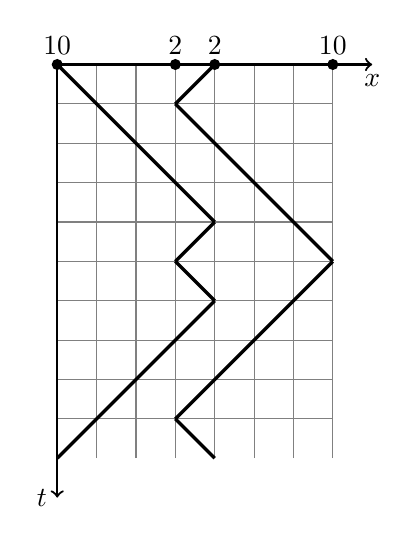
\begin{tikzpicture}
		\draw [help lines,thin,step=5mm] (0,5) grid (3.5,10);
		\draw[thick, ->] (0,10) -- (4,10) node [below] {$x$};
		\draw[thick, ->] (0,10) -- (0,4.5) node [left] {$t$};

		\fill ( 0  , 10) coordinate (c1) circle (2pt) node [above] {10};
		\fill ( 1.5, 10) coordinate (c2) circle (2pt) node [above] { 2};
		\fill ( 2  , 10) coordinate (c3) circle (2pt) node [above] { 2};
		\fill ( 3.5, 10) coordinate (c4) circle (2pt) node [above] {10};

		\draw[very thick,-] ( 0  ,10  )--( 2  , 8  );
		\draw[very thick,-] ( 2  , 8  )--( 1.5, 7.5);
		\draw[very thick,-] ( 1.5, 7.5)--( 2  , 7  );
		\draw[very thick,-] ( 2  , 7  )--( 0  , 5  );
		% \draw[very thick,-] ( 0  , 5  )--( 2  , 3  );
		% \draw[very thick,-] ( 2  , 3  )--( 1.5, 2.5);
		% \draw[very thick,-] ( 1.5, 2.5)--( 2  , 2  );
		% \draw[very thick,-] ( 2  , 2  )--( 0  , 0  );

		\draw[very thick,-] ( 2  ,10  )--( 1.5, 9.5);
		\draw[very thick,-] ( 1.5, 9.5)--( 3.5, 7.5);
		\draw[very thick,-] ( 3.5, 7.5)--( 1.5, 5.5);
		\draw[very thick,-] ( 1.5, 5.5)--( 2  , 5  );
		% \draw[very thick,-] ( 2  , 5  )--( 1.5, 4.5);
		% \draw[very thick,-] ( 1.5, 4.5)--( 3.5, 2.5);
		% \draw[very thick,-] ( 3.5, 2.5)--( 1.5, 0.5);
		% \draw[very thick,-] ( 1.5, 0.5)--( 2  , 0  );
	\end{tikzpicture}
	\caption{複数人の巡査が複雑に動く例 \label{tikz:multiserver_example}}
\end{figure}


そこでまず,この例から考えられる予想として,
各巡査の動きは,最も左を動く $s_1$ から順に
「可能な限り右に手伝いに行く」動き方(後で数学的に定義する)により貪欲決定してよいかが気になるが,
実はこれも成り立たない次のような例が存在する.
図\ref{tikz:multiserver_example2}のように,
左から $q_1 = 8$, $q_2 = 2$, $q_3 = 2$, $q_4 = 3$, $q_5 = 6$ である $5$ つの点
が存在するとき,
左図のように $s_1$ が可能な限り右に行くような動きをしてしまうと
$v_2,v_3,v_5$ の周期を満たす動きが左図のようなものになり,
$v_4$ が周期 $3$ 以内に訪問されなくなってしまうので $3$ 人目の巡査が必要になるが,
右図のようにあえて周期 $6$ で $v_1$ に戻るような動き方をすれば $2$ 人の巡査で5つの点を警備できる.


\begin{figure}[h]
	\centering
	\begin{tabular}{cc}
	
	\begin{minipage}{0.5\hsize}
		\centering
		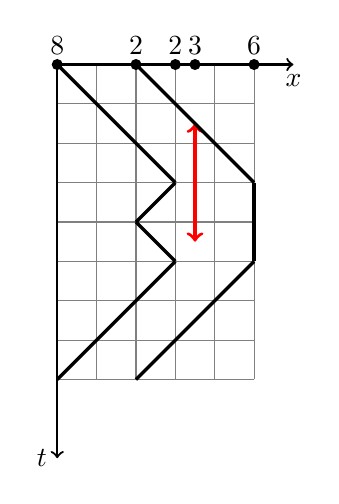
\begin{tikzpicture}
			\draw [help lines,thin,step=5mm] (0,-4) grid (2.5,0);
			\draw[thick, ->] (0,0) -- (3,0) node [below] {$x$};
			\draw[thick, ->] (0,0) -- (0,-5) node [left] {$t$};

			\fill ( 0   , 0) coordinate (c1) circle (2pt) node [above] {8};
			\fill ( 1   , 0) coordinate (c2) circle (2pt) node [above] {2};
			\fill ( 1.5 , 0) coordinate (c3) circle (2pt) node [above] {2};
			\fill ( 1.75, 0) coordinate (c4) circle (2pt) node [above] {3};
			\fill ( 2.5 , 0) coordinate (c5) circle (2pt) node [above] {6};

			\draw[very thick,red,<->] (1.75,-0.75)--(1.75,-2.25);

			\draw[very thick,-] ( 0  , 0  )--( 1.5,-1.5);
			\draw[very thick,-] ( 1.5,-1.5)--( 1  ,-2  );
			\draw[very thick,-] ( 1  ,-2  )--( 1.5,-2.5);
			\draw[very thick,-] ( 1.5,-2.5)--( 0  ,-4  );
			% \draw[very thick,-] ( 0  ,-4  )--( 1.5,-5.5);
			% \draw[very thick,-] ( 1.5,-5.5)--( 1  ,-6  );

			\draw[very thick,-] ( 1  , 0  )--( 2.5,-1.5);
			\draw[very thick,-] ( 2.5,-1.5)--( 2.5,-2.5);
			\draw[very thick,-] ( 2.5,-2.5)--( 1  ,-4  );
			% \draw[very thick,-] ( 1  ,-4  )--( 2.5,-5.5);
			% \draw[very thick,-] ( 2.5,-5.5)--( 2.5,-6  );
		\end{tikzpicture}
	\end{minipage}
	
	\begin{minipage}{0.5\hsize}
		\centering
		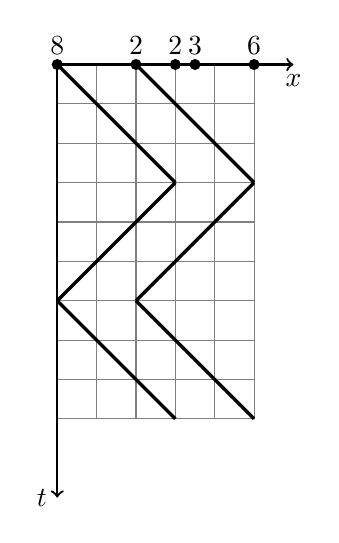
\begin{tikzpicture}
			\draw [help lines,thin,step=5mm] (0,-4.5) grid (2.5,0);
			\draw[thick, ->] (0,0) -- (3,0) node [below] {$x$};
			\draw[thick, ->] (0,0) -- (0,-5.5) node [left] {$t$};

			\fill ( 0   , 0) coordinate (c1) circle (2pt) node [above] {8};
			\fill ( 1   , 0) coordinate (c2) circle (2pt) node [above] {2};
			\fill ( 1.5 , 0) coordinate (c3) circle (2pt) node [above] {2};
			\fill ( 1.75, 0) coordinate (c4) circle (2pt) node [above] {3};
			\fill ( 2.5 , 0) coordinate (c5) circle (2pt) node [above] {6};

			\draw[very thick,-] ( 0  , 0  )--( 1.5,-1.5);
			\draw[very thick,-] ( 1.5,-1.5)--( 0  ,-3  );
			\draw[very thick,-] ( 0  ,-3  )--( 1.5,-4.5);
			% \draw[very thick,-] ( 1.5,-4.5)--( 0  ,-6  );
			\draw[very thick,-] ( 1  , 0  )--( 2.5,-1.5);
			\draw[very thick,-] ( 2.5,-1.5)--( 1  ,-3  );
			\draw[very thick,-] ( 1  ,-3  )--( 2.5,-4.5);
			% \draw[very thick,-] ( 2.5,-4.5)--( 1  ,-6  );
		\end{tikzpicture}
	\end{minipage}
	
	\end{tabular}
	\caption{「可能な限り右に手伝いに行く」戦略が失敗する例 \label{tikz:multiserver_example2}}
\end{figure}





\subsubsection{最初の訪問時刻指定,周期ちょうど毎に訪問}

各点の周期とは,2つの連続する訪問の間の時間の上限であったが,
それにより,図\ref{tikz:multiserver_example2}の例のようにあえて周期 $8$ の点を周期 $6$ で訪問
する方が良いために左端から巡査の動きを決定できないという難しさが生じてしまった.
そこで,最初の訪問時刻 $r_i$ が指定されていて,かつその時刻から毎度の訪問を周期ちょうど毎の時刻に
行わなければならないという設定を考えてみる.
すると,この設定では,左側から巡査を割り当て,「可能な限り右に行く」動き方をさせることにより
\minpatroller では最適解が得られることを以下のように示すことができる.
実際にはより一般的に,時刻 $t$ と位置 $x$ について
$t$-$x$ 平面に訪問しなければならない位置と時刻を表す点が全て与えられている問題について示される.


\begin{theo}
	\label{theo:xt_decided_1}
	各点 $x_i ( i = 1,2,\ldots,n)$ について,訪問すべき時刻の系列
	$t_{i_1},t_{i_2}, \ldots$ が指定されているとき,
	つまり,$t$-$x$ 平面に描いた巡査の軌跡が通らなければならない点の集合
	$X = \dbigcup_{i = 1}^n \dbigcup_k \set{(t_{i_k}, x_i)}$
	が与えられているとき,
	$s_1$ から順に「可能な限り右に行く動き方」で \minpatroller の最適解を得られる.
\end{theo}



\begin{defi}
	$t$-$x$ 平面において,点 $a = (t_a,x_a)$ に対して
	\begin{alignat*}{3}
	R(a)
	&:= \setmid{(t,x)}{ -x + x_a + t_a < t < x - x_a + t_a } \\
	L(a)
	&:= \setmid{(t,x)}{ (t,x) \not\in R(a) }
	\end{alignat*}
	と定義する.
	$R(a)$ を $R(t_a,x_a)$ のようにも書くことにする.
	% $t$-$x$ 平面を全体として,$R(a)$ は $L(a)$ の補集合になる.


\begin{figure}[h]
	\centering
	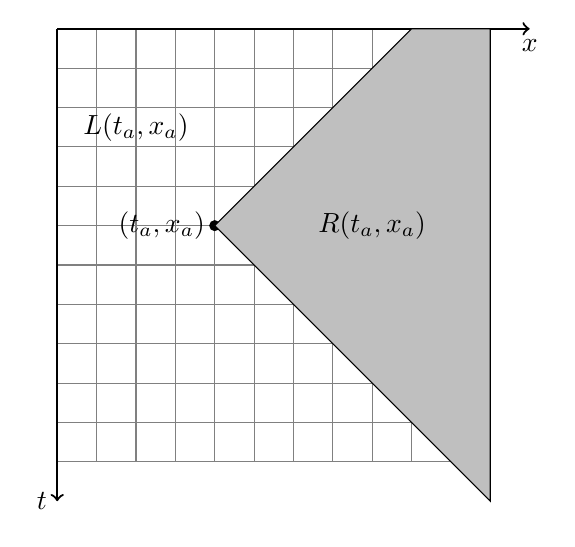
\begin{tikzpicture}
		\draw [help lines,thin,step=5mm] (0,-5.5) grid (5.5,0);
		\draw[thick, ->] (0,0) -- (6,0) node [below] {$x$};
		\draw[thick, ->] (0,0) -- (0,-6) node [left] {$t$};

		\fill ( 2,-2.5) coordinate (ab) circle (2pt) node [left] {$(t_a,x_a)$};

		\filldraw [draw=black, fill=lightgray]
			(ab)--(4.5,0)--(5.5,0)--(5.5,-6)--(ab);

		\node (L) at (1,-1.25) {$L(t_a,x_a)$};
		\node (R) at (4,-2.5) {$R(t_a,x_a)$};
	\end{tikzpicture}
	\caption{$L(t_a,x_a)$ と $R(t_a,x_a)$ の定義 \label{tikz:defLR}}
\end{figure}

\end{defi}


\begin{lemm}
	\label{lemm:xt_decided_2}
	巡査 $s$ の軌跡が $t$-$x$ 平面上のある点 $(t_a,x_a)$ を通るとき,
	$s$ の軌跡は $L(t_a,x_a)$ に含まれる ($R(t_a,x_a)$ を通らない).
\end{lemm}

\begin{proof}[Proof of \Ref{lemm:xt_decided_2}]
	$s$ の軌跡が $(t_a,x_a)$ と $(t_b,x_b) \in R(t_a,x_a)$ を通るとする.
	$(t_1, x_1) \in R$ より
	\begin{equation}
		\label{eq:lemm:xt_decided_2}
		-x_b + x_a + t_a < t_b < x_b - x_a + t_a
	\end{equation}
	が成り立つ.
	\begin{enumerate}[(i)]
		\item 
		$t_b = t_a$ のときは,式\Ref{eq:lemm:xt_decided_2}から $x_b > x_a$ となり,
		$s$ が同時に異なる2点に存在することはできないので矛盾.
		\item $t_b < t_a$ のとき,巡査の速さが1以下であることから,
		$s$ が $x = x_b$ から $x = x_a$ に移動するのには少なくとも
		$\abs{x_b - x_a} = x_b - x_a$ 時間かかるので,
		時刻 $t_b$ 以降で $x_a$ に最初に到達する時刻 $t_a$ は
		$t_a \geq t_b + x_b - x_a$ を満たすが,
		これは 式\Ref{eq:lemm:xt_decided_2}に矛盾する.
		\item $t_b > t_a$ のときも(ii)と同様.
	\end{enumerate}
	よって, $s$ は $R(t_a,x_a)$ の点を通ることはできないので,
	$s$ の軌跡は $L(t_a,x_a)$ に含まれる.
\end{proof}


$t$-$x$ 平面上の点の集合 $X'$ が与えられ,
何人かの巡査により $X'$ の点全てを通る必要があるとする.
$X' \neq \emptyset$ ならば,
巡査 $s$ を1人用意し,$X'$ を担当する巡査の中で最も左を動くものとする.
このとき,次の補題が成り立つ.


\begin{lemm}
	\label{lemm:xt_decided_2_3}
	$s$ の軌跡は $\dbigcap_{a \in X'} L(a)$ に含まれる.
\end{lemm}


\begin{proof}[Proof of \Ref{lemm:xt_decided_2_3}]
	もし $s$ の軌跡が $\dbigcup_{a \in X'} R(a)$ の点 $b = (t_b,x_b)$ を通るとすると,
	ある $a = (t_a,x_a) \in X'$ が存在して $b \in R(a)$ であるが,
	このとき補題\Ref{lemm:xt_decided_2}によると
	$s$ の軌跡は $a$ を通ることができない.
	すると,この $a$ を通る巡査 $s'$ が新たに必要になるが,
	時刻 $t_a$ において $s$ は $x \geq x_b - \abs{t_b - t_a}$ の領域に存在するため,
	\begin{itemize}
		\item $t_b < t_a$ ならば,
		式\Ref{eq:lemm:xt_decided_2}から
		$x \geq x_b - \abs{t_b - t_a} = x_b + t_b - t_a > x_a$.
		\item $t_b = t_a$ ならば,
		式\Ref{eq:lemm:xt_decided_2}から
		$x \geq x_b > x_a$.
		\item $t_b > t_a$ ならば,
		式\Ref{eq:lemm:xt_decided_2}から
		$x \geq x_b - \abs{t_b - t_a} = x_b - t_b + t_a > x_a$.
	\end{itemize}
	より,時刻 $t_b$ において $s'$ は $s$ より左に存在することになる.
	これは $s$ を最も左側にある巡査にしたことに矛盾する.
	よって,最も左側の巡査 $s$ の軌跡は
	$\dbigcup_{a \in X'} R(a)$ の点を含まないので,
	$\dbigcap_{a \in X'} L(a)$ に含まれることが言える.
\end{proof}




% \begin{figure}[h]
% 	\centering
% 	\begin{tikzpicture}
% 		% \draw [help lines,thin,step=5mm] (0,-8) grid (5.5,0);
% 		\draw[thick, ->] (0,0) -- (6,0) node [below] {$x$};
% 		\draw[thick, ->] (0,0) -- (0,-9.5) node [left] {$t$};

% 		\fill ( 2  ,-2.5) coordinate (p1) circle (2pt) node [left] {$p_1$};
% 		\fill ( 3  ,-4  ) coordinate (p2) circle (2pt) node [left] {$p_2$};
% 		\fill ( 2  ,-5.5) coordinate (p3) circle (2pt) node [left] {$p_3$};

% 		\filldraw [draw=black, fill=lightgray]
% 			(p1)--(4.5,0)--(5.5,0)--(5.5,-6)--(p1);

% 		\filldraw [draw=black, fill=lightgray]
% 			(p3)--(5.5,-2)--(5.5,-9)--(p3);

% 		\filldraw [draw=black, fill=lightgray]
% 			(p2)--(5.5,-1.5)--(5.5,-6.5)--(p2);

% 		\node (L) at (1.5,-1.5) {$\dbigcap_{a \in X'} L(a)$};
% 		\node (R) at (4,-2.5)   {$\dbigcup_{a \in X'} R(a)$};
% 	\end{tikzpicture}
% 	\caption{$L(t_a,x_a)$ と $R(t_a,x_a)$ の定義 \label{tikz:defLR}}
% \end{figure}



\begin{lemm}
	\label{lemm:xt_decided_3}
	$t$-$x$ 平面上の点の集合 $X'$ に対し,
	$\dbigcap_{a \in X'} L(a)$ の(右の)境界線上にある点の集合を
	\[
		B(X') := \setmid{ b \in X'}{ b \in \bigcap_{a \in X'} L(a) }
	\]
	と表す.
	$X'$ を訪問する巡査のうち最も左にあるものを $s$ とすると,
	$s$ はその軌跡が $\dbigcap_{a \in X'} L(a)$ の(右側の)境界と一致する動きが最適であり,
	これにより $B(X')$ の点全体を担当することができる(これを「可能な限り右に行く動き」と定義する).
\end{lemm}


\begin{proof}[Proof of \Ref{lemm:xt_decided_3}]
	補題\Ref{lemm:xt_decided_2}より,$s$ の軌跡は
	$\dbigcap_{a \in X'} L(a)$ に含まれるので,
	$s$ が通ることができる点全体は
	$B(X')$ の点の部分集合となる.
	逆に,$s$ は $B(X')$ の点全てを通ることができる.
	なぜならば, $\dbigcap_{a \in X'} L(a)$ の境界線は常に
	傾きが $\pm 1$ であるため,$B(X')$ の点のうち時刻の最も早い点から
	出発して境界線上を動くことにより
	$B(X')$ の点全てを通ることができるためである.

	また,$B(X')$ の点を全て通る動き方は最適である.
	なぜならば,$B(X')$ のうち通らない点がある場合,それらの点の集合を $X''$ と置くと,
	$X'' \cup (X' \setminus B(X'))$ の点全てを通る巡査達の動きにより
	$X' \setminus B(X')$ 全体を通ることができるので,
	$B(X')$ のうち通らない点を残すことにより得をしていないからである.
\end{proof}


以上より,定理\Ref{theo:xt_decided_1}に戻ると,
\[
X_i := 
\begin{cases}
	X & i = 1 \\
	X_{i - 1} \setminus B(X_{i - 1}) & i \geq 2
\end{cases}
\]
として,
$X_i$ が空集合になるまで $i = 1$ から順に $B(X_i)$ を巡査 $s_i$ が担当するようにすれば,
% 点全体 $X$ に対して,境界線上の点 $B(X)$ を $s_1$ が担当し,
% $X_2 \neq \emptyset$ ならば
% $B(X_2)$ の点を $s_2$ が担当し,というように
% $X$ を
最適解が得られる.
\qed \Ref{theo:xt_decided_1}.

この定理により得られた結果は
この問題設定に対しては巡査を左から可能な限り右に行く動き方で割り当てていけば良いということを
数学的に示したものであるが,
有限の手続きにより $X$ 全体を通る巡査数を求めることができるとは限らない.
なぜならば,$X$ の点が時刻$t$に関して周期的になっていない場合 $X$ は $t$ 方向に
無限に長い領域で考える必要があるため $X$ や $B(X)$ が無限集合となるためである.
$X$ を有限集合で考えてよい場合は $N := |X|$ として
以下の手順により $\Theta(N \log N)$ で
$t$-$x$ 平面上の巡査達の軌跡を描くことができる.

まず,$X$ の各点の元の $t$-$x$ 座標系での表示を
$45^\circ$ 反時計回りに回転した $u$-$y$ 座標系での表示に変換する.
すなわち,各点 $(t_i, x_i)$ を以下のように $(u_i, y_i)$ に変換する.
\begin{align*}
	\begin{pmatrix}
		u_i \\ y_i
	\end{pmatrix}
	&=
	\begin{pmatrix}
		\cos(-45^\circ) & - \sin(-45^\circ) \\
		\sin(-45^\circ) &   \cos(-45^\circ)
	\end{pmatrix}
	\begin{pmatrix}
		t_i \\ x_i
	\end{pmatrix} \\
	&=
	\frc{\sqrt{2}}
	\begin{pmatrix}
		1  & 1 \\
		-1 & 1
	\end{pmatrix}
	\begin{pmatrix}
		t_i \\ x_i
	\end{pmatrix}
\end{align*}

次にこの変換後の $N$ 点を $u$ の昇順,同着はさらに $y$ の昇順でソートする.
変換・ソート後の点を
$a_1, \ldots, a_N$  とする $( u_1 \leq u_2 \leq \cdots \leq u_N)$ .

以降,この $u$-$y$ 平面上の $N$ 点に対して,
$y$ 軸に平行な scanline を $u = u_1$ の位置から右に動かしていくことを考える.
% $a_1'$ は
% $\sforall a_i' \in \set{a_2', \ldots, a_N'} . \lr a_1' \not\in R(a_i') }$
% を満たすため,必ず最も $x$ 軸方向で左側の巡査$s_1$ の担当となる.

\begin{figure}[h]
	\centering
	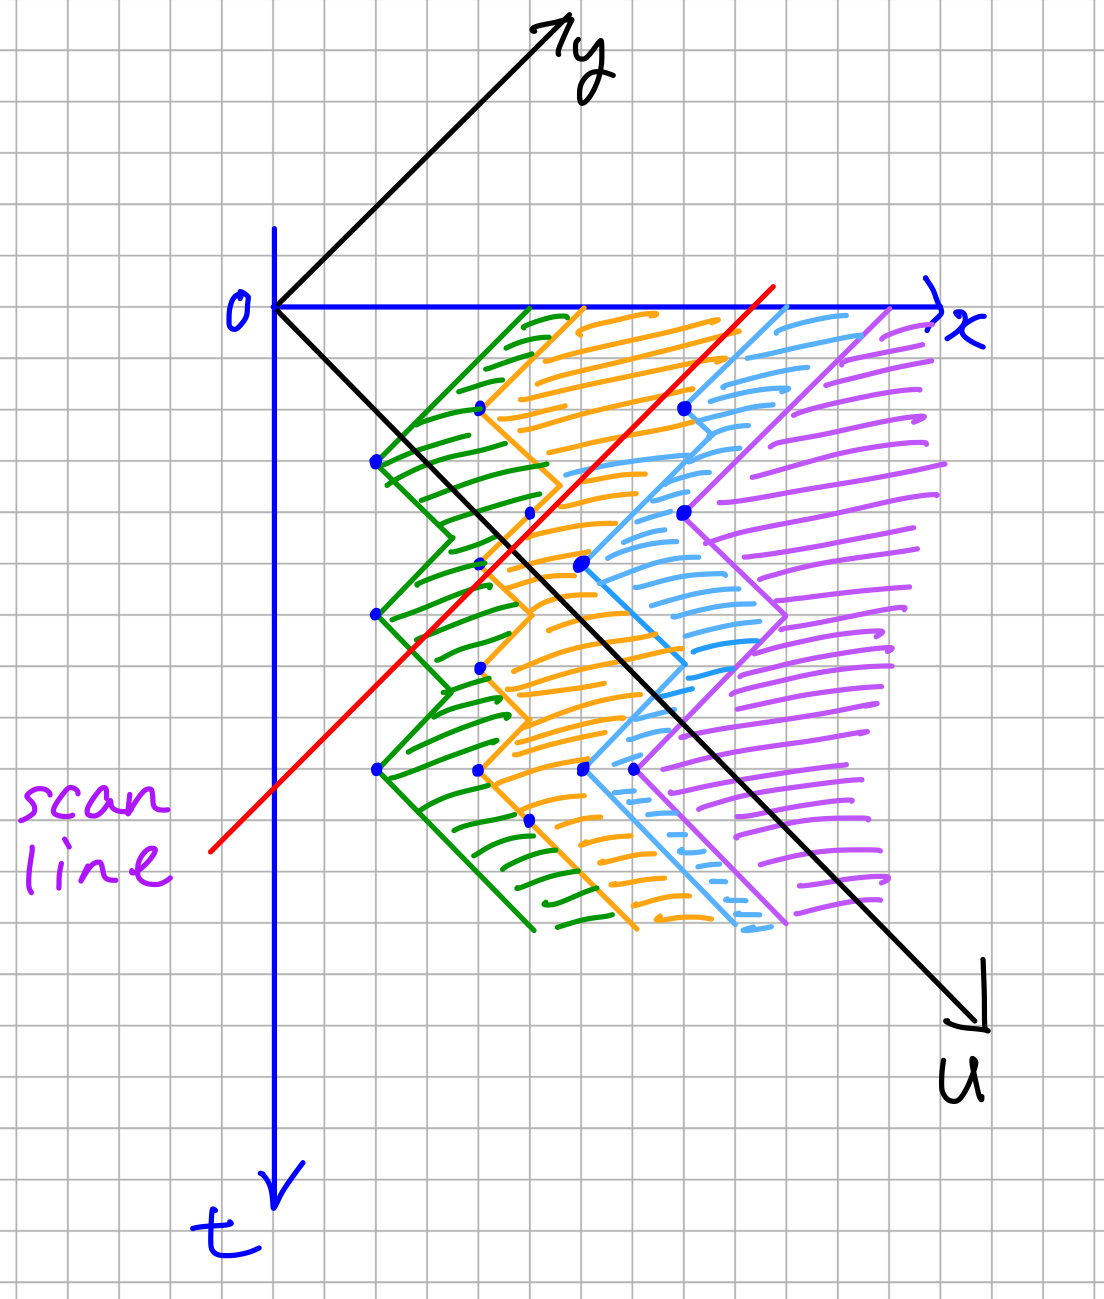
\includegraphics[width=6cm]{./figures/figure1.jpeg}
	\caption{$t$-$x$ 平面上に描いた巡査達の軌跡 \label{fig:uyspace}}
\end{figure}

初めに scanline 全体を色 $c_0$ で塗る.

scanline が $a_1$ に重なったとき,
scanline の $y > y_1$ の部分を色 $c_1$ で塗る.
次に scanline が $a_2$ に重なったとき,
$y_2$ が scanline の色 $c_0$ の範囲(境界は含まれる)にあれば
$y_2 \leq y \leq y_1$ と点 $a_2$ を色 $c_1$ で塗る.
$y_2$ が scanline の色 $c_1$ の範囲にあれば
$y \geq y_2$ と点 $a_2$ を色 $c_2$ で塗る.


このように,
scanline を動かしていって新たに重なる点 $a_i$ が scanline の
色 $c_k$ の部分にあれば,$y_i$ から色 $c_{k + 1}$ で塗られた部分まで
(無ければ $y = \infty$ まで)色 $c_{k + 1}$ で塗ることを繰り返していく.
このように点と重なるごとに更新されていく scanline の色で $t$-$x$ 平面を塗り分けていくことで
平面上のそれぞれの色 $c_i$ の領域が
$\dbigcup_{a \in B(X_i)} R(a) \setminus \dbigcup_{a \in B(X_{i + 1})} R(a)$
を表すことになり,
その境界線上を各巡査が動けばよいことが分かる.

scanline の色として説明した部分は,
scanline の色に対応する区間を管理すればよく,
平衡二分木を用いて,各点と重なる毎に $O(\log N)$ で検索・追加をすれば,
合計 $O(N \log N)$ で平面の塗り分けが完了する.
ソートと合わせて全体の計算量は $O(N \log N)$ となる.

scanline は各点を通る時点で
各点を担当する巡査の番号と軌跡が決められるので,
随時必要な情報を出力していくことができる.
これにより巡査の数を知ることができるのも明らかである.

最初に戻り,訪問間隔と最初の訪問時刻が指定された問題を考えると,
これは $lcm(q_1, \ldots, q_n)$ ( $lcm$ は最小公倍数) 周期で繰り返しとなるので
$N = \dsum_{i = 1}^n \dfrac{lcm(q_1, \ldots, q_n)}{q_i} \leq n \cdot lcm(q_1, \ldots, q_n)$
となり,擬多項式時間算法となる.

% \subsubsection{周期が異なる場合 - \maxprofit}








\section{Star}


\subsection{巡査が1人の場合}

Star は全ての辺の端点の一方が原点 $0$ である木である.
$v_i$ と原点の間の辺の長さを $d_i$ と書くことにする.

巡査1人のStar で $p_i = 1, q_i = Q$ の場合は簡単で,
周期 $Q$ を満たす範囲で原点からの辺の長さ $d_i$ が短い点を順に選んでいけば良い.

一方,$p_i$, $q_i$ のいずれかが任意の場合は NP困難となる.

\begin{theo}
	巡査1人,$G$ が Star で $q_i = Q$ の \maxprofit はNP困難である.
\end{theo}
\begin{proof}
ナップザック問題からの帰着による.

ナップザック問題とは,入力として
容量 $B$ の容器と,
品物の集合 : $I = \set{ 1, 2, \ldots, n }$ が与えられ,
各品物 $i$ のサイズが $a_i$, 利得が $w_i$ であるとき,
$I$ の部分集合 $I'$ であって
$\dsum_{ i \in I'} a_i \leq B$ を満たしながら
利得の合計 $\dsum_{i \in I'} w_i \geq W$ となるものが存在するかを判定する問題である.

この問題は巡査1人,$G$ が Star, $q_i = Q$ の \maxprofit に帰着できる.
各品物 $i$ に対して点 $v_i$ を用意し,
各辺の長さを $d_i = a_i/2$, 周期 を $q_i = B$, 利得を $p_i = w_i$ とする.

すると,ナップザック問題の解 $I'$ が与えられたとき,
$I'$ に対応する点の集合 $V'$ について
\begin{equation}
  \sum_{x_i \in V'} 2 d_i = \sum_{i \in I'} a_i \leq B
\end{equation}
より巡査は $c'$ の点を全て警備することができ,利得の合計は $W$ 以上となる.
逆に, Star の解の点集合 $V'$ が与えられたとき,
$V'$ に対応する品物集合 $I'$ は
\begin{equation}
  \sum_{i \in I'} a_i = \sum_{x_i \in V'} 2 d_i \leq B
  \qquad
  \sum_{i \in I'} w_i \geq W
\end{equation}
を満たすので,ナップザック問題の解とすることができる.
以上によりナップザック問題を帰着できたので
巡査1人,$G$ が Star, $q_i = Q$ の \maxprofit はNP困難となる.
\end{proof}





\begin{theo}
	巡査1人,$G$ が Star で $p_i = 1$ の \maxprofit はNP困難である.
\end{theo}
\begin{proof}
3-partition 問題からの帰着による.

3-partition 問題とは,入力として,
容量 $B$ の容器が $k$ 個与えられ,
サイズ $a_i$ が $B/4 < a_i < B/2$, $\sum a_i = kB$ を満たす品物が $3k$ 個与えられるとき,
$k$個の容器に $3k$個の品物を詰めることができるかを判定する問題である.
$B/4 < a_i < B/2$ という制約から品物は3個まで容器に詰めることができるが,
3個ずつ詰められた場合のみ $3k$個の品物を $k$個の容器に詰めることができる.

この問題は巡査1人,$G$ が Star で $p_i = 1$ の \maxprofit に帰着できる.
点を $3k + 1$ 個用意し,図\ref{fig:star3partitionNPhard}のように
1つの点 $v_0$ は周期 $q_0 = B + 2$, $d_0 = 1$, 
その他の点 $v_i$ は周期 $q_i = k(B + 2)$, $d_i = a_i/2$ というようにする.

\begin{figure}
	\centering
	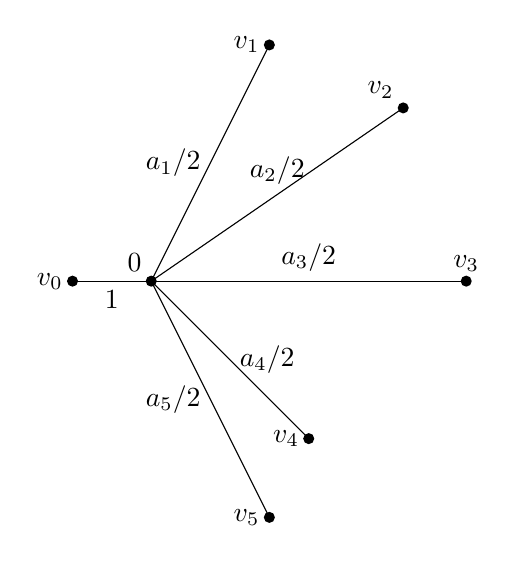
\begin{tikzpicture}
		\fill (-1,0) coordinate (cz) circle (2pt) node [left] {$v_0$};
		\fill ( 0,0) coordinate (O) circle (2pt) node [above left] {$0$};
		\draw[-] (cz) -- node[below] {1} (O);
		\fill ( 1.5, 3  ) coordinate (c1) circle (2pt) node [left] {$v_1$};
		\fill ( 3.2, 2.2) coordinate (c2) circle (2pt) node [above left] {$v_2$};
		\fill ( 4  , 0  ) coordinate (c3) circle (2pt) node [above] {$v_3$};
		\fill ( 2  ,-2  ) coordinate (c4) circle (2pt) node [left] {$v_4$};
		\fill ( 1.5,-3  ) coordinate (c5) circle (2pt) node [left] {$v_5$};
		\draw[-] (O) -- node[left ] {$a_1/2$} (c1);
		\draw[-] (O) -- node[above] {$a_2/2$} (c2);
		\draw[-] (O) -- node[above] {$a_3/2$} (c3);
		\draw[-] (O) -- node[right] {$a_4/2$} (c4);
		\draw[-] (O) -- node[left ] {$a_5/2$} (c5);
	\end{tikzpicture}
	\caption{3-Partitionの帰着 \label{fig:star3partitionNPhard}}
\end{figure}

すると,3-partition が可能なときは,Star で $v_0$ からスタートし,
各容器に詰める3個ずつの品物に対応する点を3つ訪問して$v_0$ に戻るという巡回を
することにより,各点の周期 を満たしながら全点を警備することができる.

逆に, Star で全点を警備できるとき,
巡査は$v_0$ を訪問した後3つの異なる点を選んで訪問し $v_0$ に戻ってくるということを
$k$ 回繰り返している必要がある.
なぜならば,$v_0$ の周期 は $B + 2$ なので原点までの行き帰り分の2を引くと
点までの道のりを $B$ まで走ることができるが,$B/4 < a_i$ という条件から高々3つの点しか
訪問することはできず,
逆に2つ以下しか訪問せずに $v_0$ に戻ることがあるとすると, $a_i < B/2$ より
全点を1周するまでに $k + 1$ 回以上 $v_0$ に戻る必要があり,
その時間は $kB + 2(k + 1)$ 以上となるため,
各点の周期 $k(B + 2)$ を満たすことができないからである.
よって,全点を1周できたときにはちょうど3個ずつの点 $k$ 組に分割できたことになるので
3-partitionの解となる.

以上により3-partition問題を帰着できたので,
巡査1人,$G$ が Star で $p_i = 1$ の \maxprofit はNP困難となる.
\end{proof}




\subsection{巡査が複数の場合}
Star の複数の巡査による警邏問題は全てNP困難となる.
これは以下の定理により示される.

\begin{theo}
	$G$ が Star で $p_i = 1$, $q_i = Q$ の \minpatroller はNP困難である.
	\label{theo:minpatroller_Star_NPhard}
\end{theo}

\begin{proof}
Partition からの帰着による.
Partition は,入力としてある正の値の集合
$X = \set{ a_1, \ldots, a_n }$ が与えられたとき,
これを
$X_1 \cap X_2 = \emptyset$, $X_1 \cup X_2 = X$,
$\dsum_{a_i \in X_1} a_i = \dsum_{a_i \in X_2} a_i =: k$
を満たすように分割できるかを判定する問題である.

これは $G$ が Star, $p_i = 1$, $q_i = Q$ の \minpatroller に帰着できる.
先ほどの Partition の入力に対し,
サイズ $n$ の点の集合 $V = \set{ v_1, \ldots, v_n }$ を考え,
各 $v_i$ について $d_i = a_i / 2$, $q_i = k$ というようにする.

Partition が Yes の場合,
$X_1$ と $X_2$ に対応する点集合を $s_1$, $s_2$ がそれぞれ警邏することにより
全点を警備できる.

逆に \minpatroller で巡査数が2となれば,
それぞれが周期 $k$ をちょうど満たしながら共通部分のない2つの点部分集合を巡回していることになる.

全ての点は少なくとも1回はこの時間に訪問されなければならない.
すると,各点 $v_i \in V$ に対して
$[t_0, t_0 + Q]$ のうち少なくとも $a_i$ の時間は
$v_i$ に対応する辺 $e_i$ に巡査は存在しなければならないことを以下のように示せる.

時間 $[t_0, t_0 + Q]$ に少なくとも1回 $v_i \in V$ はいずれかの巡査により訪問される.
\begin{itemize}
	\item
	ある巡査が時間 $[t_0 + a_i/2, t_0 + Q - a_i/2]$ に $v_i$ を
	1度でも訪問しているとき(いずれかの巡査が $v_i$ に存在する時刻が
	$[t_0 + a_i/2, t_0 + Q - a_i/2]$ の中にあるとき),
	少なくともその前後 $a_i$ の時間はその巡査は辺 $e_i$ 上に存在しなければならず,
	この時間は $[t_0, t_0 + Q]$ に含まれている.
	\item 
	$v_i$ が $[t_0 + a_i/2, t_0 + Q - a_i/2]$ に1度も訪問されないときは,
	$[t_0, t_0 + a_i/2)$ または $(t_0 + Q - a_i/2, t_0 + Q]$ に少なくとも1度訪問される.
	$[t_0, t_0 + a_i/2)$ に訪問される場合,点 $v_i$ に巡査が存在した
	最後の時刻を $t_e \in [t_0, t_0 + a_i/2)$ とすると,
	$t_e + Q$ までに再び $v_i$ は訪問されるはずである.
	$[t_e, t_0 + Q - a_i/2]$ に再び訪問されることはない場合を考えているので,
	再度訪問される時刻は $[t_0 + Q - a_i/2, t_e + Q]$ に含まれることになる.
	すると,巡査は $[t_0, t_e + a_i/2] \cup [t_e + Q - a_i/2, t_0 + Q]$ の時間は
	辺 $e_i$ に存在することになるので,
	$[t_0, t_0 + Q]$ の間に合計で少なくとも
	$(t_e + a_i/2 - t_0) + (t_0 + Q - (t_e + Q - a_i/2)) = a_i$ の時間
	巡査は辺 $e_i$ に存在することになる.
	$(t_0 + Q - a_i/2, t_0 + Q]$ の場合も対称なので同様に考えればよい.
\end{itemize}
これにより,巡査は訪問のために合計 $\dsum a_i = 2Q$ の時間を使わねばならず,
またそれぞれの巡査が使える時間は $Q$ なので,2人の巡査により全点を警備しているならば
同じ点を $s_1$ と $s_2$ の両方が警備することはないので,
巡査 $s_1$, $s_2$ の警備する集合 $V_{s_1}$, $V_{s_2}$ 
がそれぞれ $X$ の分割 $X_1$, $X_2$ となり Partition は Yes となる.

以上によりPartition問題を帰着できたので
$G$ が Star, $p_i = 1$, $q_i = Q$ の \minpatroller はNP困難である.
\end{proof}






\section{StarC}

Star については $d_i$ が任意ではなく一定とした場合も考えてみる.
Star では巡査1人で $p_i = 1$, $q_i = Q$ の \maxprofit
では多項式時間算法が存在し,他はNP困難となったが,
StarC の場合は $q_i = Q$ の場合には全て多項式時間算法が存在する.


\subsection{巡査が1人の場合}

この場合は周期が全て等しいならば多項式時間で解くことができる.

\begin{itemize}
\item 
$q_i = Q$ のときは全ての点の訪問のコストが等しいので,
$p_i$ の大きいものから選ぶことで最適解が得られる.
$p_i$ をソートして上位から $\lrfloor{\dfrac{Q}{2d}}$ 個の点を選ぶだけなので,
ヒープソートを用いれば $O\lr{n + \lrfloor{\dfrac{Q}{2d}} \log n}$ の時間で解くことができる.

\item 
$p_i = 1$ のときは $q_i$ の大きいものから選ぶことで,
警備できる点の数を最大化できる.
なぜならば,
警備している点の集合 $V_s$ について,
$x_i \in V_s$ と $x_j \in V \setminus V_s$ であって
$q_i < q_j$ となる組が存在すれば,
辺の長さが全て同じなので $x_i$ を訪問する時間で代わりに $x_j$ を訪問することができ,
$q_i < q_j$ であるからそれ以外の時間は元の巡査の動きをそのまま用いることができるためである.
こうして得られる警備する点の集合 $V_s \cup \set{ x_j} \setminus \set{ x_i }$ の利得は
元の利得以上となる.
しかし,$q_i$ の大きいものからいくつ選べるかは自明ではなく,未解決.

\item 
$p_i$ も $q_i$ も定数でない場合も未解決.
\end{itemize}




\subsubsection{最初の訪問時刻指定,周期ちょうど毎に訪問}

Line のときのように,
StarC で未解決の部分について,最初の訪問時刻と訪問間隔の指定された問題をここでも考えてみる.


\begin{theo}
	巡査1人, $G$ が StarC, $p_i = 1$, 
	最初の訪問時刻 $r_i$ と訪問間隔 $q_i$ の指定された \maxprofit はNP困難である.
\end{theo}


\begin{proof}
	独立点集合問題からの帰着による.

	独立点集合問題は,
	無向グラフ $G' = (V', E')$ と自然数 $M$ が与えられたときに
	独立点集合
	$V_I = \setmid{ v' \in V' }
	{ \sforall v_i', v_j' \in V_I . (v_i', v_j') \not\in E'}$
	でサイズ $|V_I|$ が $M$ 以上のものが存在するかを判定する問題である.

	この問題において, 2点間に辺の存在する $v_i, v_j \in V'$ を両方選ぶことはできないということを,
	\maxprofit において2点のどちらか一方しか警備できないという状況を作ることで表現する.

	まず簡単のため $d = 1/2$ とする.
	これにより巡査がちょうど速さ $1$ で動くとすると各点の訪問にかかる時間は $1$ となり,
	Star なので全ての整数の時刻にどれか1点を訪問できる.
	その上で,$q_i$, $r_i$ は整数であるとする.
	\maxprofit の StarC の点集合 $V$ は $V'$ のサイズと同じとし,以降同じ添え字で対応させる.
	点 $v_i \in V$ を警備するために訪問しなければならない時刻の系列は
	$q_i k + r_i \; (k \in \N)$ で表される.
	すると, $v_i$ と $v_j$ の両方を警備できる必要十分条件は
	$q_i k + r_i = q_j l + r_j$ , 移項すると
	$r_i - r_j = q_j l - q_i k$ 
	となる自然数 $k, l$ が存在しないこととなるが,
	これは $r_i - r_j = gcd(q_i,q_j) n$ となる整数 $n$ が存在しないことと同値である.
	実際,
	$r_i - r_j = q_j l - q_i k$ となる自然数 $k,l$ が存在するとき,
	$gcd(a,b)$ を $a$ と $b$ の最大公約数として,
	$n = \dfrac{q_j}{gcd(q_i,q_j)} l - \dfrac{q_i}{gcd(q_i,q_j)} k$ とすれば
	$r_i - r_j = gcd(q_i,q_j) n$ であり,
	逆に $r_i - r_j = gcd(q_i,q_j) n$ となる整数 $n$ が存在するとき,
	$gcd(q_i,q_j) = q_i l' + q_j k'$ を満たす整数の組 $l'$, $k'$ が存在することは
	ユークリッド互除法より言えるので, $l = nl'$, $k = -nk'$ とすると
	$r_i - r_j = q_j l - q_i k$ となる.
	まとめると, $v_i$ と $v_j$ の両方を警備できる必要十分条件は
	\begin{equation}
		r_i \not\equiv r_j \mod gcd(q_i, q_j)
	\end{equation}
	となる.

	ここで,$\dbinom{n}{2}$ 個の相異なる素数 $p_{ij} (1\leq i < j \leq n)$ を用意し,
	各点の周期を
	\begin{align*}
		q_i
		&= \lr{\prod_{j = 1, \ldots, i - 1} p_{ji}}
		   \lr{\prod_{j = i + 1 \ldots, n} p_{ij}} \\
		&= p_{1i} p_{2i} \cdots p_{(i - 1)i} p_{i(i + 1)} \cdots p_{i,n}
	\end{align*}
	とすると,$gcd(q_i,q_j) = p_{ij}$ ($i < j$ のとき)となり,
	先ほどの条件は
	\begin{equation}
		r_i \not\equiv r_j \mod p_{ij}
	\end{equation}
	となる.

	$G'$ において
	$(v_i', v_j') \in E'$     ならば $r_i \equiv r_j \equiv 0 \mod p_{ij}$,
	$(v_i', v_j') \not\in E'$ ならば $r_i \equiv 0, r_j \equiv 1 \mod p_{ij}$
	と定めると,
	各 $r_k$ に対して相異なる $n - 1$ 個の素数で割ったときのあまりが与えられるので,
	中国剰余定理からそのような $r_k$ が一意に存在することが言え,
	$(v_i', v_j') \in E'$ ならば $r_i \equiv r_j \mod p_{ij}$
	$(v_i', v_j') \not\in E'$ ならば $r_i \not\equiv r_j \mod p_{ij}$
	を満たすように各 $r_k$ を定めることができた.

	最後に,$\dbinom{n}{2}$ 個の相異なる素数を用意する計算が多項式時間で可能かが問題だが,
	${\bf TODO!!!}$ 

	以上の手順で $q_k$ と $r_k$ を設定することにより,
	$G'$ においてサイズ $M$ 以上の独立点集合が存在するかという問題を,
	巡査1人, $G$ が StarC, $p_i = 1$,
	最初の訪問時刻 $r_i$ と訪問間隔 $q_i$ の指定された \maxprofit において
	総利得 $M$ 以上の警邏が存在するかという問題に帰着できた.
	以上より定理は示された
\end{proof}






\subsection{巡査が複数の場合}

Star の複数人の巡査による警邏はNP困難であったが,
StarC の場合周期が全て等しいならば多項式時間算法が存在する.

この場合,点の訪問のコストが全て等しいことから,
利得の大きいものから選べばよいことは明らかであるが,
ちょうど $\lrfloor{\dfrac{mQ}{2d}}$ 点を警備する警邏を以下のように構成できる.

まず,利得の大きいものから $\lrfloor{\dfrac{mQ}{2d}} (=: l)$ 点を求め,
$v_1', v_2', \ldots, v_l'$ とする 
$(p_1' \geq p_2' \geq \cdots \geq p_l')$.

最初に巡査 $s_1$ が時刻 $t_0$ に原点を出発して
$v_1', v_2', \ldots, v_l'$ を順番に速さ$1$ で動きながら訪問していく.
巡査 $s_i$ は時刻 $t_0 + (i - 1)Q$ に原点を出発し,
$s_1$ より $(i - 1)Q$ だけ遅れて同じ動きをする.
各巡査が原点を出発して $v_1', \ldots, v_l'$ を訪問し
再び原点に戻るまでの時間は $2dl$ であり,
$2dl = 2d \lrfloor{\dfrac{mQ}{2d}} \leq mQ$ であるから,
時刻 $t_0 + (i - 1)Q$ に原点を出発した巡査 $s_i$ は
時刻 $t_0 + (i - 1)Q + mQ$ までには $v_l'$ まで訪問して原点に戻っており,
時刻 $t_0 + (i - 1)Q + mQ$ に原点を出発して再び同じ動きを繰り返すことができる.

このような動きを繰り返すことで,どの点 $v_i'$ についてもちょうど $Q$ おきに
巡査が訪問しているため,$v_1, \ldots, v_l'$ を警備できている.


一方,$m$ 人の巡査が警備できる点は高々 $\lrfloor{\dfrac{mQ}{2d}}$ 点である.
任意の長さ $Q$ の時間 $[t_0, t_0 + Q]$ を切り取って考える.
点集合 $V_S \subseteq V$ の点を全て警備しているとき,
$V_S$ の全ての点は少なくとも1回はこの時間に訪問されなければならない.
すると,各点 $v_i \in V_S$ に対して
$[t_0, t_0 + Q]$ のうち少なくとも $2d$ の時間は
$v_i$ に対応する辺 $e_i$ に巡査は存在しなければならないことを
定理 \ref{theo:minpatroller_Star_NPhard} のときと同様に示せる.

% 任意の点 $v_i \in V_S$ について,
% 時間 $[t_0, t_0 + Q]$ に少なくとも1回 $v_i$ はいずれかの巡査により訪問される.
% \begin{itemize}
% \item
% ある巡査が時間 $[t_0 + d, t_0 + Q - d]$ に $v_i$ を
% 1度でも訪問しているとき(いずれかの巡査が $v_i$ に存在する時刻が
% $[t_0 + d, t_0 + Q - d]$ の中にあるとき),
% 少なくともその前後 $2d$ の時間はその巡査は辺 $e_i$ 上に存在しなければならず,
% またこの時間は $[t_0, t_0 + Q]$ に含まれている.
% \item 
% $v_i$ が $[t_0 + d, t_0 + Q - d]$ に1度も訪問されないときは,
% $[t_0, t_0 + d)$ または $(t_0 + Q - d, t_0 + Q]$ に少なくとも1度訪問される.
% $[t_0, t_0 + d)$ に訪問される場合,点 $v_i$ に巡査が存在した
% 最後の時刻を $t_e \in [t_0, t_0 + d)$ とすると,
% $t_e + Q$ までに再び $v_i$ は訪問されるはずである.
% $[t_e, t_0 + Q - d]$ に再び訪問されることはない場合を考えているので,
% 再度訪問される時刻は $[t_0 + Q - d, t_e + Q]$ に含まれることになる.
% すると,巡査は $[t_0, t_e + d] \cup [t_e + Q - d, t_0 + Q]$ の間は
% 辺 $e_i$ に存在することになるので,
% $[t_0, t_0 + Q]$ の間に合計で少なくとも
% $(t_e + d - t_0) + (t_0 + Q - (t_e + Q - d)) = 2d$ の時間
% 巡査は辺 $e_i$ に存在することになる.
% $(t_0 + Q - d, t_0 + Q]$ の場合も対称なので同様に考えればよい.
% \end{itemize}
% 以上により示された.

% すると, $m$ 人の巡査で $V_S$ の点を訪問するとき
% 巡査が使える時間は合計 $mQ$ であるので,
% $2d \cdot |V_S| \leq mQ$ である必要があり,
% これにより $|V_S| \leq \lrfloor{\dfrac{mQ}{2d}}$ が言える.

以上から $\lrfloor{\dfrac{mQ}{2d}}$ 点の警邏が最適解であることが分かる.
よって,巡査が1人のときと同様にして
$O\lr{n + \lrfloor{\dfrac{mQ}{2d}} \log n}$ の時間で解くことができる.


% \section{Tree}




\section{一般のグラフ}
Star で巡査数 $1$, $p_i = 1$, $q_i = Q$ の最も簡単な場合以外は全てNP困難となったので,
一般のグラフについては $p_i = 1$, $q_i = Q$ の場合のみが問題となるが,これはNP困難となる.

\begin{theo}
	巡査が1人, $G$ が一般のグラフ, $p_i = 1$, $q_i = Q$ の \maxprofit はNP困難である.
\end{theo}
\begin{proof}
ハミルトン閉路問題からの帰着による.

ハミルトン閉路問題とは,入力としてグラフ $G' = (V',E')$ が与えられたときに,
全点をちょうど1回訪れる巡回が存在するかを判定する問題である.

これは巡査が1人, $G$ が一般のグラフ, $p_i = 1$, $q_i = Q$ の \maxprofit に帰着できる.
まずグラフ $G$ を元に完全グラフ $G = (V,E)$ で,$V = V'$, 
$E$ の各辺 $e_{ij}$ についてその長さが
\begin{equation}
d_{ij} =
\begin{cases}
	1 & \IF e_{ij} \in E \\
	2 & \IF e_{ij} \not\in E
\end{cases}
\end{equation}
であるものを考え,$p_i = 1$, $q_i = |V|$ とする.

すると,利得 $|V|$ が得られる警邏が存在するかを判定する問題は,
長さ $1$ の辺のみを動いて全点を警備できるかの判定に相当するので,
ハミルトン閉路問題と同値となる.

以上によりハミルトン閉路問題を帰着できたので,
巡査が1人, $G$ が一般のグラフ, $p_i = 1$, $q_i = Q$ の \maxprofit はNP困難である.
\end{proof}

さらに $d$ を平面上のユークリッド距離とする部分問題も
巡回セールスマン問題からの帰着により NP困難であることが示される.






% \section{問題設定の拡張}
\section{拘束時間}
点の訪問時に一定時間巡査が待機しなければならないという問題設定も考えられる.

拘束時間 $w_i$ が $0$ でないときは,
元のグラフの点の位置から長さ $w_i / 2$ の枝を生やしてその末端に点を配置し
拘束時間無しとした問題に変換できる.
すると,元の問題で全ての点が1点に集まっている場合($v_1 = v_2 = \cdots = v_n$)でも
変換後のグラフがStarとなるので,
拘束時間無しのStarでの結果から任意の形状について,
巡査が1人では $p_i$, $q_i$ いずれかが定数でない場合は NP困難,
巡査が複数では $p_i = 1, q_i = Q$ でも NP困難と分かる.

巡査1人で $p_i = 1, q_i = Q$ の \maxprofit は,
拘束時間付きの Line は変換後は木となるが,
木については巡査1人で $p_i = 1, q_i = Q$ の場合
多項式時間算法が存在することが分かっている~\cite{coene2013balancing}.
StarC, Star は Star に変換されるので多項式時間で最適解が与えられる.





\section{ToDo}
\begin{itemize}
	\item 図のサイズ調整など,全8ページ以内になるように
	\item 手書きをtikzに
\end{itemize}


